% !TeX root = ..//diffgeo_main.tex
\begin{defs}[Differenzierbare Mannigfaltigkeit]
Eine \textit{differenzierbare Struktur} auf einer topologischen Mannigfaltigkeit $\mfk$ ist ein \textit{maximaler $C^\infty$-Atlas}. Eine \textit{differenzierbare Mannigfaltigkeit} ist eine topologische Mannigfaltigkeit mit einer differenzierbaren Struktur.
\end{defs}

\begin{bem}
Man kann auch eine topologische Mannigfaltigkeit definieren, ohne das 2. Abzählbarkeitsaxiom zu fordern.
\begin{description}
\item[Aber:] Dann bekommt man Mannigfaltigen mit ganz anderen Eigenschaften als diejenigen, die wir betrachten wollen.
\item[Wichtig:] Hausdorffsch + 2. Abzählbarkeitsaxiom $\Rightarrow$ parakompakt, d. h. jede offene Überdeckung hat eine lokal endliche Verfeinerung.
\end{description}
$(V_j)$ heißt Verfeinerung von $(U_i)$, falls $\forall V_j \exists U_i$ mit $V_j \subseteq U_i$\\
Lokal endlich: $\forall p \in X\ \exists$ Umgebung $U$, die nur endlich viele $V_j$ trifft\\
Parakompakt $\Rightarrow \exists$ Partition der Eins f mit 
\begin{align*}
f_i: V_i \subseteq X \rightarrow [0, 1],\ \sum_{i \in I} f_i (x) = 1
\end{align*} 
\end{bem}

\begin{bsp}
Metrische Räume sind parakompakt.
\end{bsp}

\begin{bsp}[differenzierbare Mannigfaltigkeiten]
\begin{enumerate}
\item$\mathbb{R}^n$ mit Atlas $\mathcal{A} = \{(\operatorname{id}, \R^n)\}$
\item$V$ Vektorraum, $B$ Basis mit $B = \{v_1, \cdots, v_n\}$, Atlas $\mathcal{A} = \set{(\chi_B, V)}$
\begin{align*}
& \chi_B: V \rightarrow \R^n\\
& v = \sum^n_{i=1} a_i v_i \mapsto \sum_{i=1}^n a_i e_i
\end{align*}
wobei $(e_1, \cdots, e_n)$ die Standardbasis ist.
\item$\mfk \subseteq \R^n,\ (\chi_U, U)$ mit $\chi_U = \operatorname{id}\vert_U,\ V \subseteq \mfk^n,\ M$ differenzierbare Mannigfaltigkeit, $\mathcal{A} = \set{(\chi_U, U)}$ Atlas von $\mfk$\\
$\mathcal{A}_V = \set{(\chi_V, U_V}$ wobei $(\chi_V, U_V) = (\chi_{U\cap V}, U\cap V)$
\item$\mfk_1 = S^1,\ M_2 = \R,\ M_1\times \mfk_2 =$ "unendlicher Zylinder"

\hspace{.06\textwidth}
\begin{minipage}[H]{0.8\textwidth}
Seien $M_1^{n_1}, M_1^{n_2}$ differenzierbare Mannigfaltigkeiten, so ist $M_1\times M_2$ ebenfalls eine \difM \ der Dimension $n_1 + n_2$.\\
Atlas $\mathcal{A} = \set{(x\times y, U\times V)}$, wobei 
\begin{align*}
(x, U) &= \text{Karte von } M_1\\
(y, V) &= \text{Karte von } M_2
\end{align*}
$(x\times y)(p_1, p_2) = (x(p_1), y(p_2))$
\end{minipage}
\hspace{1cm}
\begin{minipage}[H]{.2\textwidth}
\vspace{-1.5cm}
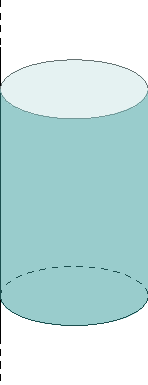
\includegraphics[scale=0.5]{figures/tikz/cylinder.pdf}
\end{minipage}

\item $S_R^n = \{ (x_0, \dots, x_n) \in \R^{n+1} \vert \sum_{i=0}^n x_i^2 = R^2 \} \subset \R^{n+1}$

\begin{itemize}
\item Teilraumtopologie: $U \subset S^n_R$ offen $\Leftrightarrow \exists U' \subset \R^{n+1}$ offen mit $U = U' \cap S^n_R$
\item Atlas: Wir brauchen zwei Karten. 
Einmal für den Nord- und einmal für den Südpol (haben unterschiedliche Orientierung).  \\
Nordpol ($N$):
\begin{align}
f_N : S^n_R \backslash \{ N \} \to \rn \\
f_N (x_0, \dots , x_n) = \frac{R}{R- x_0} (x_1, \dots, x_n) 
\end{align}
Analog für den Südpol (S):
\begin{align}
f_S : \mfk_s \to \rn
\end{align}
\end{itemize}
$\to$ Zwei Karten $f_N$ und $f_S$ ("Stereographische Projektionen").
\begin{figure}[H]
\centering
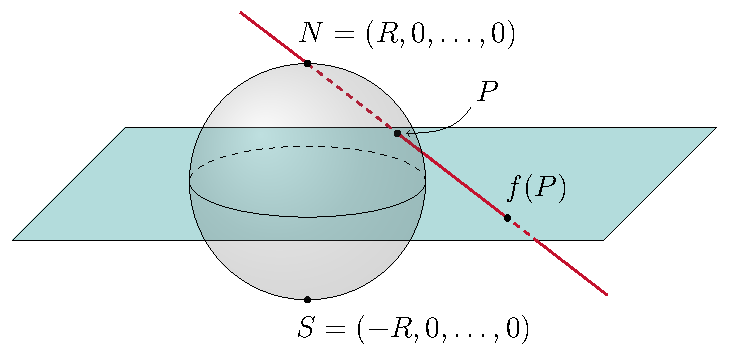
\includegraphics[scale=0.8]{figures/tikz/stereographic_projection.pdf}
\end{figure}
\end{enumerate}
\end{bsp}

\begin{bem}
$N$ mit der Teilraumtopologie und dem Atlas $\mathcal{A}_N = \set{(\chi\vert_U, U\cap N)}$ ist eine \difM.
\end{bem}

\begin{defs}
Seien $\mfk, \mfka$ differenzierbare Mannigfaltigkeiten. Eine \textit{Einbettung} ist eine differenzierbare Abbildung
\begin{align*}
f: \mfka \rightarrow \mfk
\end{align*}
sodass
\begin{enumerate}
\item$f(N)\subset M$ eine Untermannigfaltigkeit 
\item$f: N \rightarrow f(N)$ Diffeomorphismus
\end{enumerate}
\end{defs}

\section{Differenzierbare Abbildungen}
\begin{defs}[Differenzierbare Abbildungen]
Seien $\mfk$, $\mfka$ differenzierbare Mannigfaltigkeiten. 
Eine Abbildung $f: \mfk \to \mfka$ heißt differenzierbar, falls $\forall p \in \mfk$ Karten $(x, U)$ von $\mfk$ um $p$ (Karten $(y, V)$ von $\mfka$ um $f(p)$)
\end{defs}
Es gilt: $y \circ f \circ x^{-1}: x(U \cap f^{-1} (U')) \to y(f(U) \cap U')$ ist $\cinf$-differenzierbar.
Wir bezeichnen die Menge aller differenzierbaren Abbildungen durch $\cinf(\mfk, \mfka)$; $\mathcal{F}(\mfk) = \cinf(\mfk, \R)$.

\begin{defs}[Diffeomorphismus]
Eine differenzierbare Abbildung $f: \mfk \to \mfka$ heißt Diffeomorphismus, falls f eine Bijektion und $f^{-1}$ differenzierbar ist. \\
Die Menge aller Diffeomorphismes $f: \mfk \to \mfka$ bezeichnen wir mit $\diff(\mfk, \mfka)$
$\diff(\mfk) \equiv \diff(\mfk, \mfka)$ bilden eine Gruppe (Diffeomorphismengruppe).
\end{defs}


\section{Untermannigfaltigkeiten}

\begin{defs}[Untermannigfaltigkeiten]
Sei $\mfk$ eine differenzierbare Mannigfaltigkeit. 
Eine Teilmenge $\mfka \subseteq \mfk$ heißt Untermannigfaltigkeit falls:
$\forall p \in \mfka \exists$ Karte $(x, U)$ von $\mfk$ um p $x: \mfk \to V' \times V''$ mit $x(\mfk \cap \mfka) = V' \times \{z_0 \}$
für ein $z_0 \in V''$
\end{defs}


\begin{bem}
$\mfka$ mit der Teilraumtopologie und dem Atlas $\atlas_\mfka = \{ (x_U, U \cap \mfka ) \}$ ist eine differenzierbare Mannigfaltigkeit.
\end{bem}

\begin{defs}[Einbettung]
Seien $\mfk$, $\mfka$ differenzierbare Mannigfaltigkeiten. 
Eine Einbettung ist eine differenzierbare Abbildung
\begin{align}
f: \mfk \to \mfka 
\end{align}
Sodass
\begin{itemize}
\item $f(\mfka) \cap \mfk$ eine Umkehrfunktion.
\item $f: \mfka \to f(\mfka)$ Diffeomorphismus.
\end{itemize}
\end{defs}


\section{Tangentialraum} 

%\missingfigure{Tangentialräume}

\begin{defs}
\begin{enumerate}
\item Ein Tangentialvektor an $\mfk$ im Punkt $p \in \mfk$ ist eine $\R$-lineare Abbildung
\begin{align*}
v: \mathcal{F}(\mfk) \rightarrow \R
\end{align*}
mit $v(fg) = v(f)g(p) + f(p)v(g)$.
\item Die Menge aller Tangentialvektoren an $\mfk$ in $p$ heißt \textit{Tangentialraum} von $\mfk$ in $p$: $T_p \mfk$\\
$T_p \mfk$ ist ein Vektorraum.
\end{enumerate}

\begin{figure}[H]
\centering
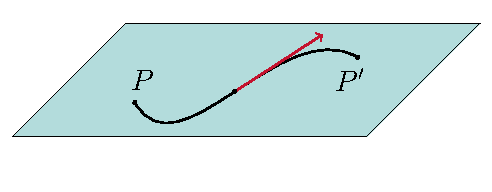
\includegraphics[scale=1]{figures/tikz/tangentline.pdf}
\end{figure}
\end{defs}
